\documentclass{article}
\usepackage[margin=1in]{geometry}
\usepackage{amsmath,amsthm,amssymb}
\usepackage{bbm,enumerate,mathtools}
\usepackage{tikz,pgfplots}
\usepackage{chessboard}
\usepackage[hidelinks]{hyperref}
\usepackage{multicol} % Problem 35
\usepackage{xstring} % Difficulty command
\usetikzlibrary{shapes.geometric}

\newenvironment{question}{\begin{trivlist}\item[\textbf{Question.}]}{\end{trivlist}}
\newenvironment{note}{\begin{trivlist}\item[\textbf{Note.}]}{\end{trivlist}}
\newenvironment{references}{\begin{trivlist}\item[\textbf{References.}]}{\end{trivlist}}
\newenvironment{related}{\begin{trivlist}\item[\textbf{Related.}]\end{trivlist}\begin{enumerate}}{\end{enumerate}}

\newcommand\score[1]{
\pgfmathsetmacro\pgfxa{#1+1}
\tikzstyle{scorestars}=[
  star,
  star points=5,
  star point ratio=2.25,
  draw,
  inner sep=3pt,
  anchor=outer point 5
]
  \begin{tikzpicture}[baseline]
    \draw[opacity=0] (0,-0.5) rectangle (0,0.2); % Workaround for whitespace at the bottom.
    \foreach \i in {1,...,4} {
      \pgfmathparse{(\i<=#1?"yellow":"gray")}
      \edef\starcolor{\pgfmathresult}
      \draw (\i*4.5ex,0) node[name=star\i,scorestars,fill=\starcolor]  {};
    }
  \end{tikzpicture}
}

\newcommand{\difficulty}[1]{%
  \IfEqCase{#1}{%
      {1}{
        
\begin{tikzpicture}[scale=0.7, baseline=0.9mm]%
          \definecolor{slopegreen}{rgb}{0.0, 0.5, 0.0}%
          \fill[slopegreen] (0.5,0.5) circle (0.5);%
        \end{tikzpicture}%
      }%
      {2}{
        
\begin{tikzpicture}[scale=0.7, baseline=0.9mm]%
          \definecolor{slopeblue}{rgb}{0.0, 0.44, 1.00}
          \fill[slopeblue] (0,0) rectangle (1,1);%
        \end{tikzpicture}%
      }%
      {3}{
\begin{tikzpicture}[scale=0.7, baseline=0.9mm]\fill (0,0.5)--(0.5, 0)--(1,0.5)--(0.5,1)--cycle; \end{tikzpicture}}%
      {4}{
\begin{tikzpicture}[scale=0.7, baseline=0.9mm]\fill (0.25,0)--(0,0.5)--(0.25,1)--(0.5,0.5)--cycle; \fill (0.75,0)--(0.5,0.5)--(0.75,1)--(1,0.5)--cycle;\end{tikzpicture}}%
      % you can add more cases here as desired
  }[\PackageError{difficulty}{Undefined difficulty level: #1}{}]%
}%
\newcommand{\rating}[2]{\difficulty{#1}\\\score{#2}\\}


\begin{document}
\rating{3}{3}
  Consider a puzzle that consists of an $n \times n$ grid with $n$ marked cells.
  The goal of the puzzle is to partition the grid into $n$-cell regions of
  size $n$, each containing exactly one marked cell.
\begin{figure}[ht!]
  \centering
  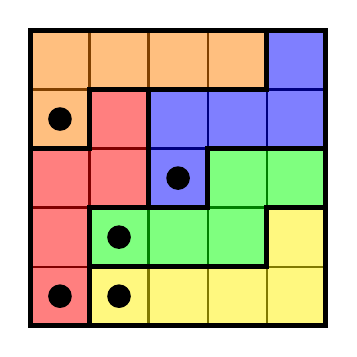
\begin{tikzpicture}[scale = 0.75]
    \draw[thick] (0,0) grid (5,5);
    \draw[fill=red, fill opacity=0.5, line width=2] (0,0)--(0,3)--(1,3)--(1,4)--(2,4)--(2,2)--(1,2)--(1,0)--cycle;
    \draw[fill=orange, fill opacity=0.5, line width=2] (0,3)--(0,5)--(4,5)--(4,4)--(1,4)--(1,3)--cycle;
    \draw[fill=yellow, fill opacity=0.5, line width=2] (1,0)--(5,0)--(5,2)--(4,2)--(4,1)--(1,1)--cycle;
    \draw[fill=green, fill opacity=0.5, line width=2] (1,1)--(4,1)--(4,2)--(5,2)--(5,3)--(3,3)--(3,2)--(1,2)--cycle;
    \draw[fill=blue, fill opacity=0.5, line width=2] (2,2)--(3,2)--(3,3)--(5,3)--(5,5)--(4,5)--(4,4)--(2,4)--cycle;

    \fill
      (0.5, 0.5) circle (0.2)
      (1.5, 0.5) circle (0.2)
      (1.5, 1.5) circle (0.2)
      (0.5, 3.5) circle (0.2)
      (2.5, 2.5) circle (0.2)
    ;
  \end{tikzpicture}
  \caption{An example of a $5 \times 5$ grid with a unique solution.}
\end{figure}

\begin{figure}[ht!]
  \centering
  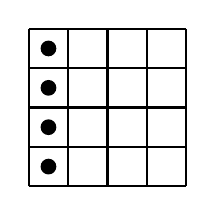
\begin{tikzpicture}[scale = 0.5]
    \draw[thick] (0,0) grid (4,4);
    \fill
      (0.5, 0.5) circle (0.2)
      (0.5, 1.5) circle (0.2)
      (0.5, 2.5) circle (0.2)
      (0.5, 3.5) circle (0.2)
    ;
  \end{tikzpicture}
  ~
  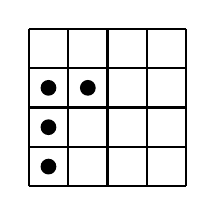
\begin{tikzpicture}[scale = 0.5]
    \draw[thick] (0,0) grid (4,4);
    \fill
      (0.5, 0.5) circle (0.2)
      (0.5, 1.5) circle (0.2)
      (0.5, 2.5) circle (0.2)
      (1.5, 2.5) circle (0.2)
    ;
  \end{tikzpicture}
  ~
  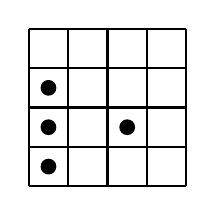
\begin{tikzpicture}[scale = 0.5]
    \draw[thick] (0,0) grid (4,4);
    \fill
      (0.5, 0.5) circle (0.2)
      (0.5, 1.5) circle (0.2)
      (0.5, 2.5) circle (0.2)
      (2.5, 1.5) circle (0.2)
    ;
  \end{tikzpicture}
  ~
  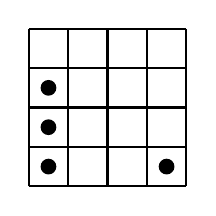
\begin{tikzpicture}[scale = 0.5]
    \draw[thick] (0,0) grid (4,4);
    \fill
      (0.5, 0.5) circle (0.2)
      (0.5, 1.5) circle (0.2)
      (0.5, 2.5) circle (0.2)
      (3.5, 0.5) circle (0.2)
    ;
  \end{tikzpicture}
  ~
  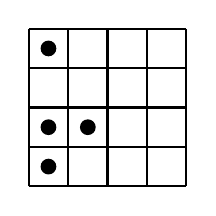
\begin{tikzpicture}[scale = 0.5]
    \draw[thick] (0,0) grid (4,4);
    \fill
      (0.5, 0.5) circle (0.2)
      (0.5, 1.5) circle (0.2)
      (1.5, 1.5) circle (0.2)
      (0.5, 3.5) circle (0.2)
    ;
  \end{tikzpicture}
  ~
  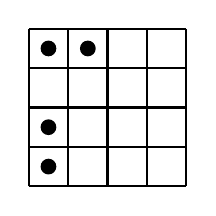
\begin{tikzpicture}[scale = 0.5]
    \draw[thick] (0,0) grid (4,4);
    \fill
      (0.5, 0.5) circle (0.2)
      (0.5, 1.5) circle (0.2)
      (1.5, 3.5) circle (0.2)
      (0.5, 3.5) circle (0.2)
    ;
  \end{tikzpicture}
  ~
  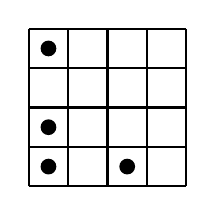
\begin{tikzpicture}[scale = 0.5]
    \draw[thick] (0,0) grid (4,4);
    \fill
      (0.5, 0.5) circle (0.2)
      (0.5, 1.5) circle (0.2)
      (2.5, 0.5) circle (0.2)
      (0.5, 3.5) circle (0.2)
    ;
  \end{tikzpicture}
  \\~\\
  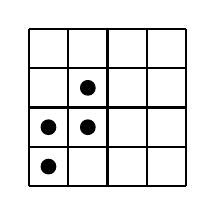
\begin{tikzpicture}[scale = 0.5]
    \draw[thick] (0,0) grid (4,4);
    \fill
      (0.5, 0.5) circle (0.2)
      (0.5, 1.5) circle (0.2)
      (1.5, 1.5) circle (0.2)
      (1.5, 2.5) circle (0.2)
    ;
  \end{tikzpicture}
  ~
  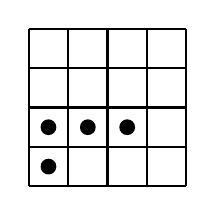
\begin{tikzpicture}[scale = 0.5]
    \draw[thick] (0,0) grid (4,4);
    \fill
      (0.5, 0.5) circle (0.2)
      (0.5, 1.5) circle (0.2)
      (1.5, 1.5) circle (0.2)
      (2.5, 1.5) circle (0.2)
    ;
  \end{tikzpicture}
  ~
  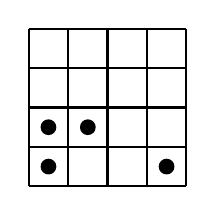
\begin{tikzpicture}[scale = 0.5]
    \draw[thick] (0,0) grid (4,4);
    \fill
      (0.5, 0.5) circle (0.2)
      (0.5, 1.5) circle (0.2)
      (1.5, 1.5) circle (0.2)
      (3.5, 0.5) circle (0.2)
    ;
  \end{tikzpicture}
  ~
  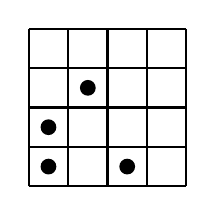
\begin{tikzpicture}[scale = 0.5]
    \draw[thick] (0,0) grid (4,4);
    \fill
      (0.5, 0.5) circle (0.2)
      (0.5, 1.5) circle (0.2)
      (1.5, 2.5) circle (0.2)
      (2.5, 0.5) circle (0.2)
    ;
  \end{tikzpicture}
  ~
  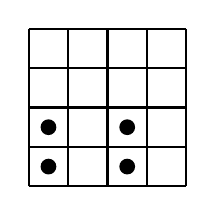
\begin{tikzpicture}[scale = 0.5]
    \draw[thick] (0,0) grid (4,4);
    \fill
      (0.5, 0.5) circle (0.2)
      (0.5, 1.5) circle (0.2)
      (2.5, 0.5) circle (0.2)
      (2.5, 1.5) circle (0.2)
    ;
  \end{tikzpicture}
  ~
  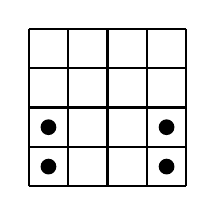
\begin{tikzpicture}[scale = 0.5]
    \draw[thick] (0,0) grid (4,4);
    \fill
      (0.5, 0.5) circle (0.2)
      (0.5, 1.5) circle (0.2)
      (3.5, 0.5) circle (0.2)
      (3.5, 1.5) circle (0.2)
    ;
  \end{tikzpicture}
  ~
  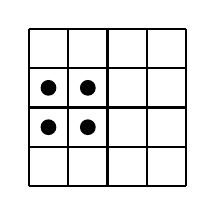
\begin{tikzpicture}[scale = 0.5]
    \draw[thick] (0,0) grid (4,4);
    \fill
      (0.5, 1.5) circle (0.2)
      (0.5, 2.5) circle (0.2)
      (1.5, 1.5) circle (0.2)
      (1.5, 2.5) circle (0.2)
    ;
  \end{tikzpicture}
  \caption{Fourteen (all, up to dihedral action?) markings with exactly one solution.}
\end{figure}

\begin{question}
  How many $n \times n$ boards exist with a unique solution? Up to dihedral action?
\end{question}

\begin{related}
  \item How many $n \times n$ boards exist with no solution? Multiple solutions?
  \item What board has the most solutions?
  \item What if this is done on an $n \times m$ board with $k$ marked cells where
    $k | nm$ and each region has $nm/k$ cells?
  \item What if the board is a torus? Triangular/hexagonal grid? Multiple dimensions?
  \item What if instead of marked cells there are marked regions?
  \item What if cells must must be rectangular? Symmetric?
  \item What if every region must be a walk starting at a marked cell?
    (As in the example.)
\end{related}

\begin{references}
  \item Problem 24
  \item \url{https://math.stackexchange.com/q/3072735/121988}
  \item \url{https://codegolf.stackexchange.com/q/179074/53884}
  \item \url{https://en.wikipedia.org/wiki/Flow_Free}
\end{references}

\end{document}
